\documentclass{beamer}
\usepackage{transparent}
\usepackage[beamer]{shortcut}


\usepackage{animate}
\usepackage{bibentry}
\usepackage{subcaption}
\usepackage{appendixnumberbeamer}

\graphicspath{{../thesis/figures/},{./images/}}
\def\TikzLocation{./tikz/}
\def\tkzscl{1}

\def\twocols{}
%\def\bimplies{}
%\def\partintro{}


\definecolor{primary}{RGB}{191,213,219}
\definecolor{secondary}{RGB}{144,106,66}
\setbeamercolor{block title}{fg=darkred}
\newcommand{\btitle}[1]{{\usebeamerfont{block title}\usebeamercolor[fg]{block title} #1}}

\AtBeginSection[]
{
}


\makeatletter
\def\beamer@newblock{%
  \usebeamercolor[fg]{bibliography entry author}%
  \usebeamerfont{bibliography entry author}%
  \usebeamertemplate{bibliography entry author}%
  \def\newblock{%
    \usebeamercolor[fg]{bibliography entry title}%
    \usebeamerfont{bibliography entry title}%
    \usebeamertemplate{bibliography entry title}%
    \def\newblock{%
      \usebeamercolor[fg]{bibliography entry location}%
      \usebeamerfont{bibliography entry location}%
      \usebeamertemplate{bibliography entry location}%
      \def\newblock{%
        \usebeamercolor[fg]{bibliography entry note}%
        \usebeamerfont{bibliography entry note}%
        \usebeamertemplate{bibliography entry note}}}}%
  \leavevmode\setbox\beamer@tempbox=\hbox{}\ht\beamer@tempbox=0em\box\beamer@tempbox}
  \setbeamertemplate{bibliography entry title}{}{}

\makeatother

\usepackage[square, authoryear]{natbib}


%-----------------------------------------------------------------------------
%	CUSTOM COMANDS
%-----------------------------------------------------------------------------

\def\keypoint#1{\hspace{0pt plus 1 filll}\textcolor{gray}{#1}}
\def\mycite#1{\keypoint{\small\citep{#1}}}
\def\citeconf#1#2{
    {\textcolor{gray}[}%
        {\color{linkcolor}\citealt{#1}, #2}%
    {\textcolor{gray}]}}
\def\citeconfright#1#2{\hspace{0pt plus 1 filll}{\small\citeconf{#1}{#2}}}
\def\biblio{
	\nobibliography{../../library}
	\def\biblio{}
}




%\usepackage{lxfonts}

\institute{-- INRIA -- Université Paris Saclay}
\author{Thomas Moreau}
\title{Distributed Convolutional Dictionary Learning (DiCoDiLe):\\Pattern Recognition in Large Signals}


\setbeamertemplate{title page}[frame]


\begin{document}

\begin{frame}[plain]
\titlepage
\biblio{}
\end{frame}

\def\biblio{}


\subfile{motiv}


%========================================================================
%\section{Scaling up Convolutional Sparse Coding with coordinate descent and distributed optimization}
%\label{sec:lgcd}
%%========================================================================
%
%\parttitleframe{Moreau2018, Moreau2019}
\subfile{dicod}


%===========================================================================
\section{Conclusion}
%===========================================================================

\begin{frame}{Conclusion}
    \textbf{Convolutional Dictionary Learning}
    \begin{itemize}\itemsep.5em
        \item Flexible pattern extraction technique,
        \item Computationally tractable for more and more problems,
        \item Some application are already beginning to emerge.
    \end{itemize}
    \vskip2em
    \textbf{Challenges}
    \begin{itemize}\itemsep.5em
        \item Theoretical challenges remains (convergence, recoverability),
        \item The evaluation (and thus the parameter choices) is still not clear,
        \item Can give some insight for deep learning models?
    \end{itemize}
\end{frame}


\begin{frame}{}
\vskip2em
{\centering
    \usebeamercolor[fg]{title}
    \usebeamerfont{title}
    \Huge \bf Thanks!\\[2em]}

Code available online:\\[1em]

%
\includegraphics[height=.8em]{github}~\textbf{LISTA} : github.com/tommoral/AdaptiveOptim\\[1em]

\includegraphics[height=.8em]{github}~\textbf{DiCoDiLe} : \url{github.com/tommoral/dicodile}\\[1em]

\includegraphics[height=.8em]{github}~\textbf{alphacsc} :  \url{alphacsc.github.io}\\[2em]

Slides are on my web page:\\[1em]
\hskip5em\includegraphics[height=.8em]{website} \url{tommoral.github.io}
\hskip4em 
\includegraphics[height=.8em]{twitter} \href{https://twitter.com/tomamoral}{@tomamoral}


\end{frame}
%===========================================================================
% AUXILIARY SLIDES
%===========================================================================



%===========================================================================
\appendix
\section{Auxiliary Slides}
%===========================================================================


%===========================================================================
\subsection{Physiological Signals}
%===========================================================================

\begin{frame}{Signals from human walking}
\centering
\vskip1em
\begin{tabular}{m{8em} m{20em}}
    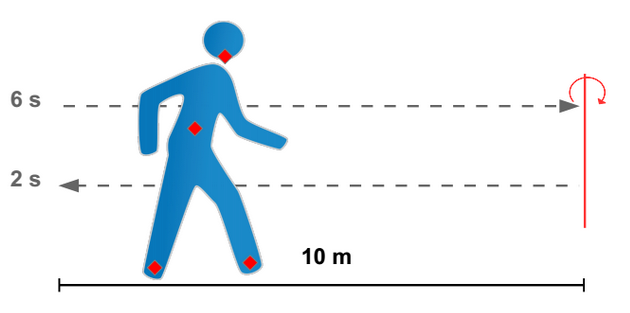
\includegraphics[width=.3\textwidth]{exo_marche}
    \raisebox{-.5\height}{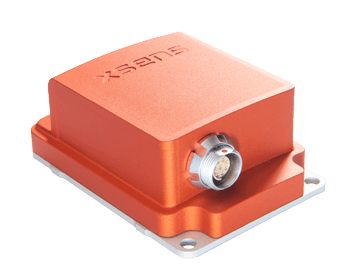
\includegraphics[width=.15\textwidth]{xsens}} $\substack{\text{Inertial}\\\text{captor}}$ &
    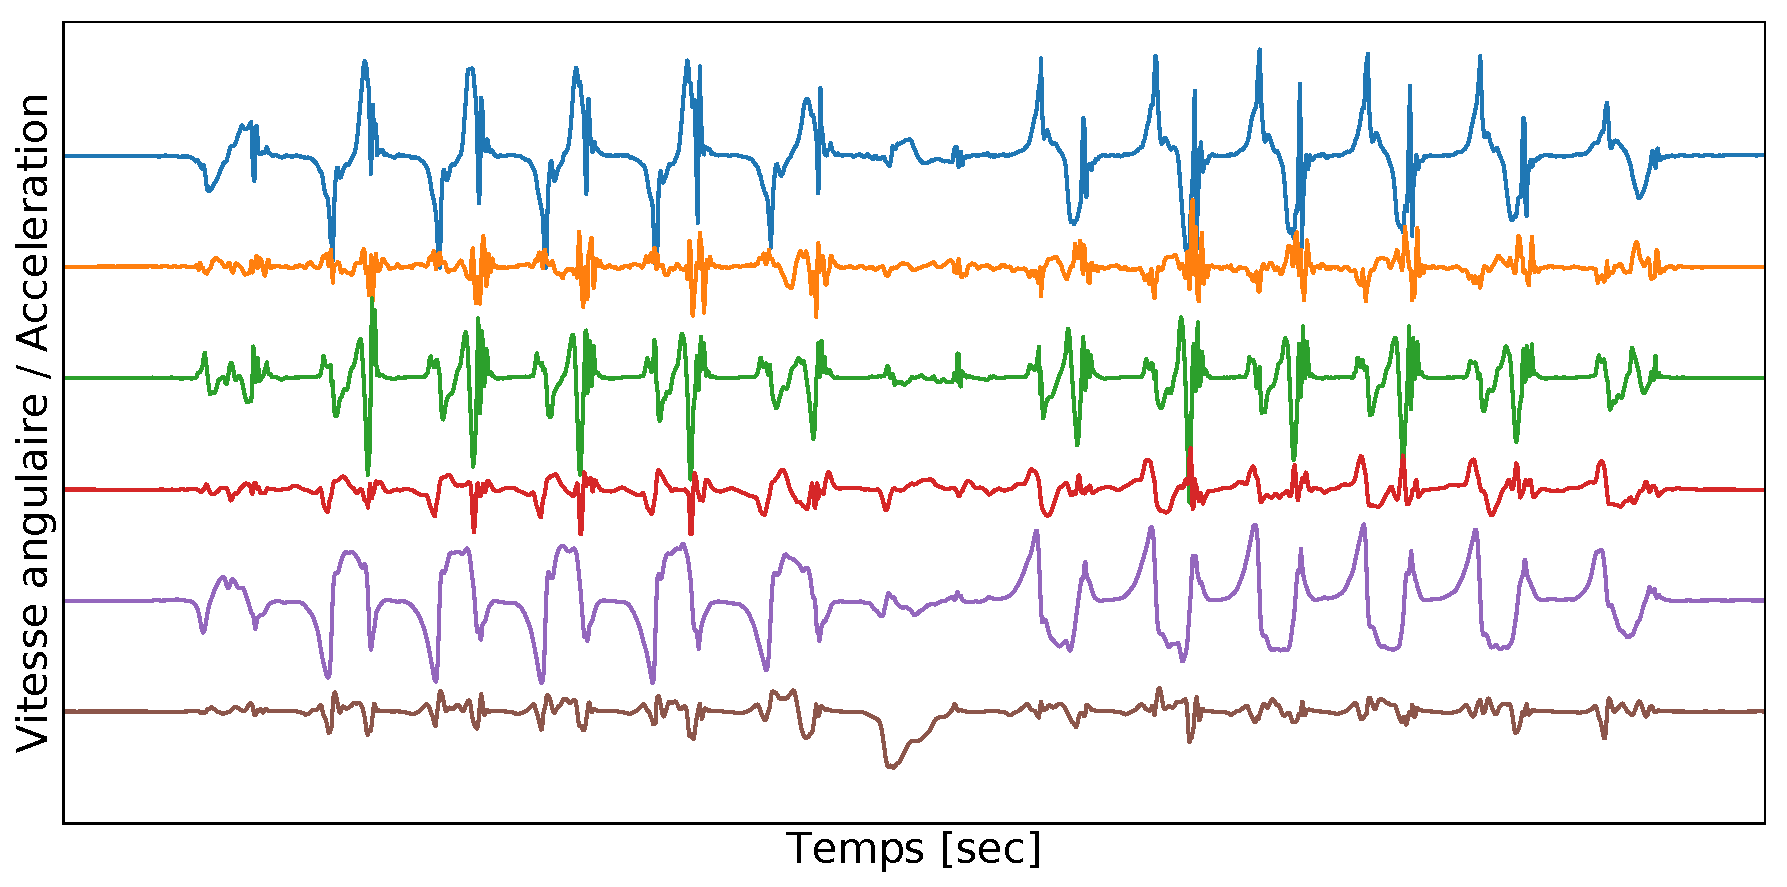
\includegraphics[width=.6\textwidth]{accelero}
\end{tabular}
\vskip1em
\begin{itemize}
    \item Shift invariant patterns linked to steps,
    \item Manual segmentation of the signal is expensive.
\end{itemize}
\strongpoint{Can we do better with data-driven approach?}

\end{frame}



\begin{frame}{Experiment}
		Create a dictionary with 25 Gaussian patterns ($W=90$)
		\[
			\pmb D^{(0)}_k \sim \mathcal N(0, I_{90})
		\]
		\vskip1em
		Use the Convolutional Dictionary Learning with\\
		DICOD to learn a dictionary $\pmb D$ on a set of $50$\\
		recording of healthy subjects walking.
		\vskip2em
		\btitle{Challenges}
		\vskip.5em
		\begin{itemize}\itemsep.5em
			\item Alignment of the patterns,
			\item Detect steps of different amplitude,
			\item Handle multivariate signals.
		\end{itemize}

\end{frame}
\begin{frame}{Experiment}
		\centering
		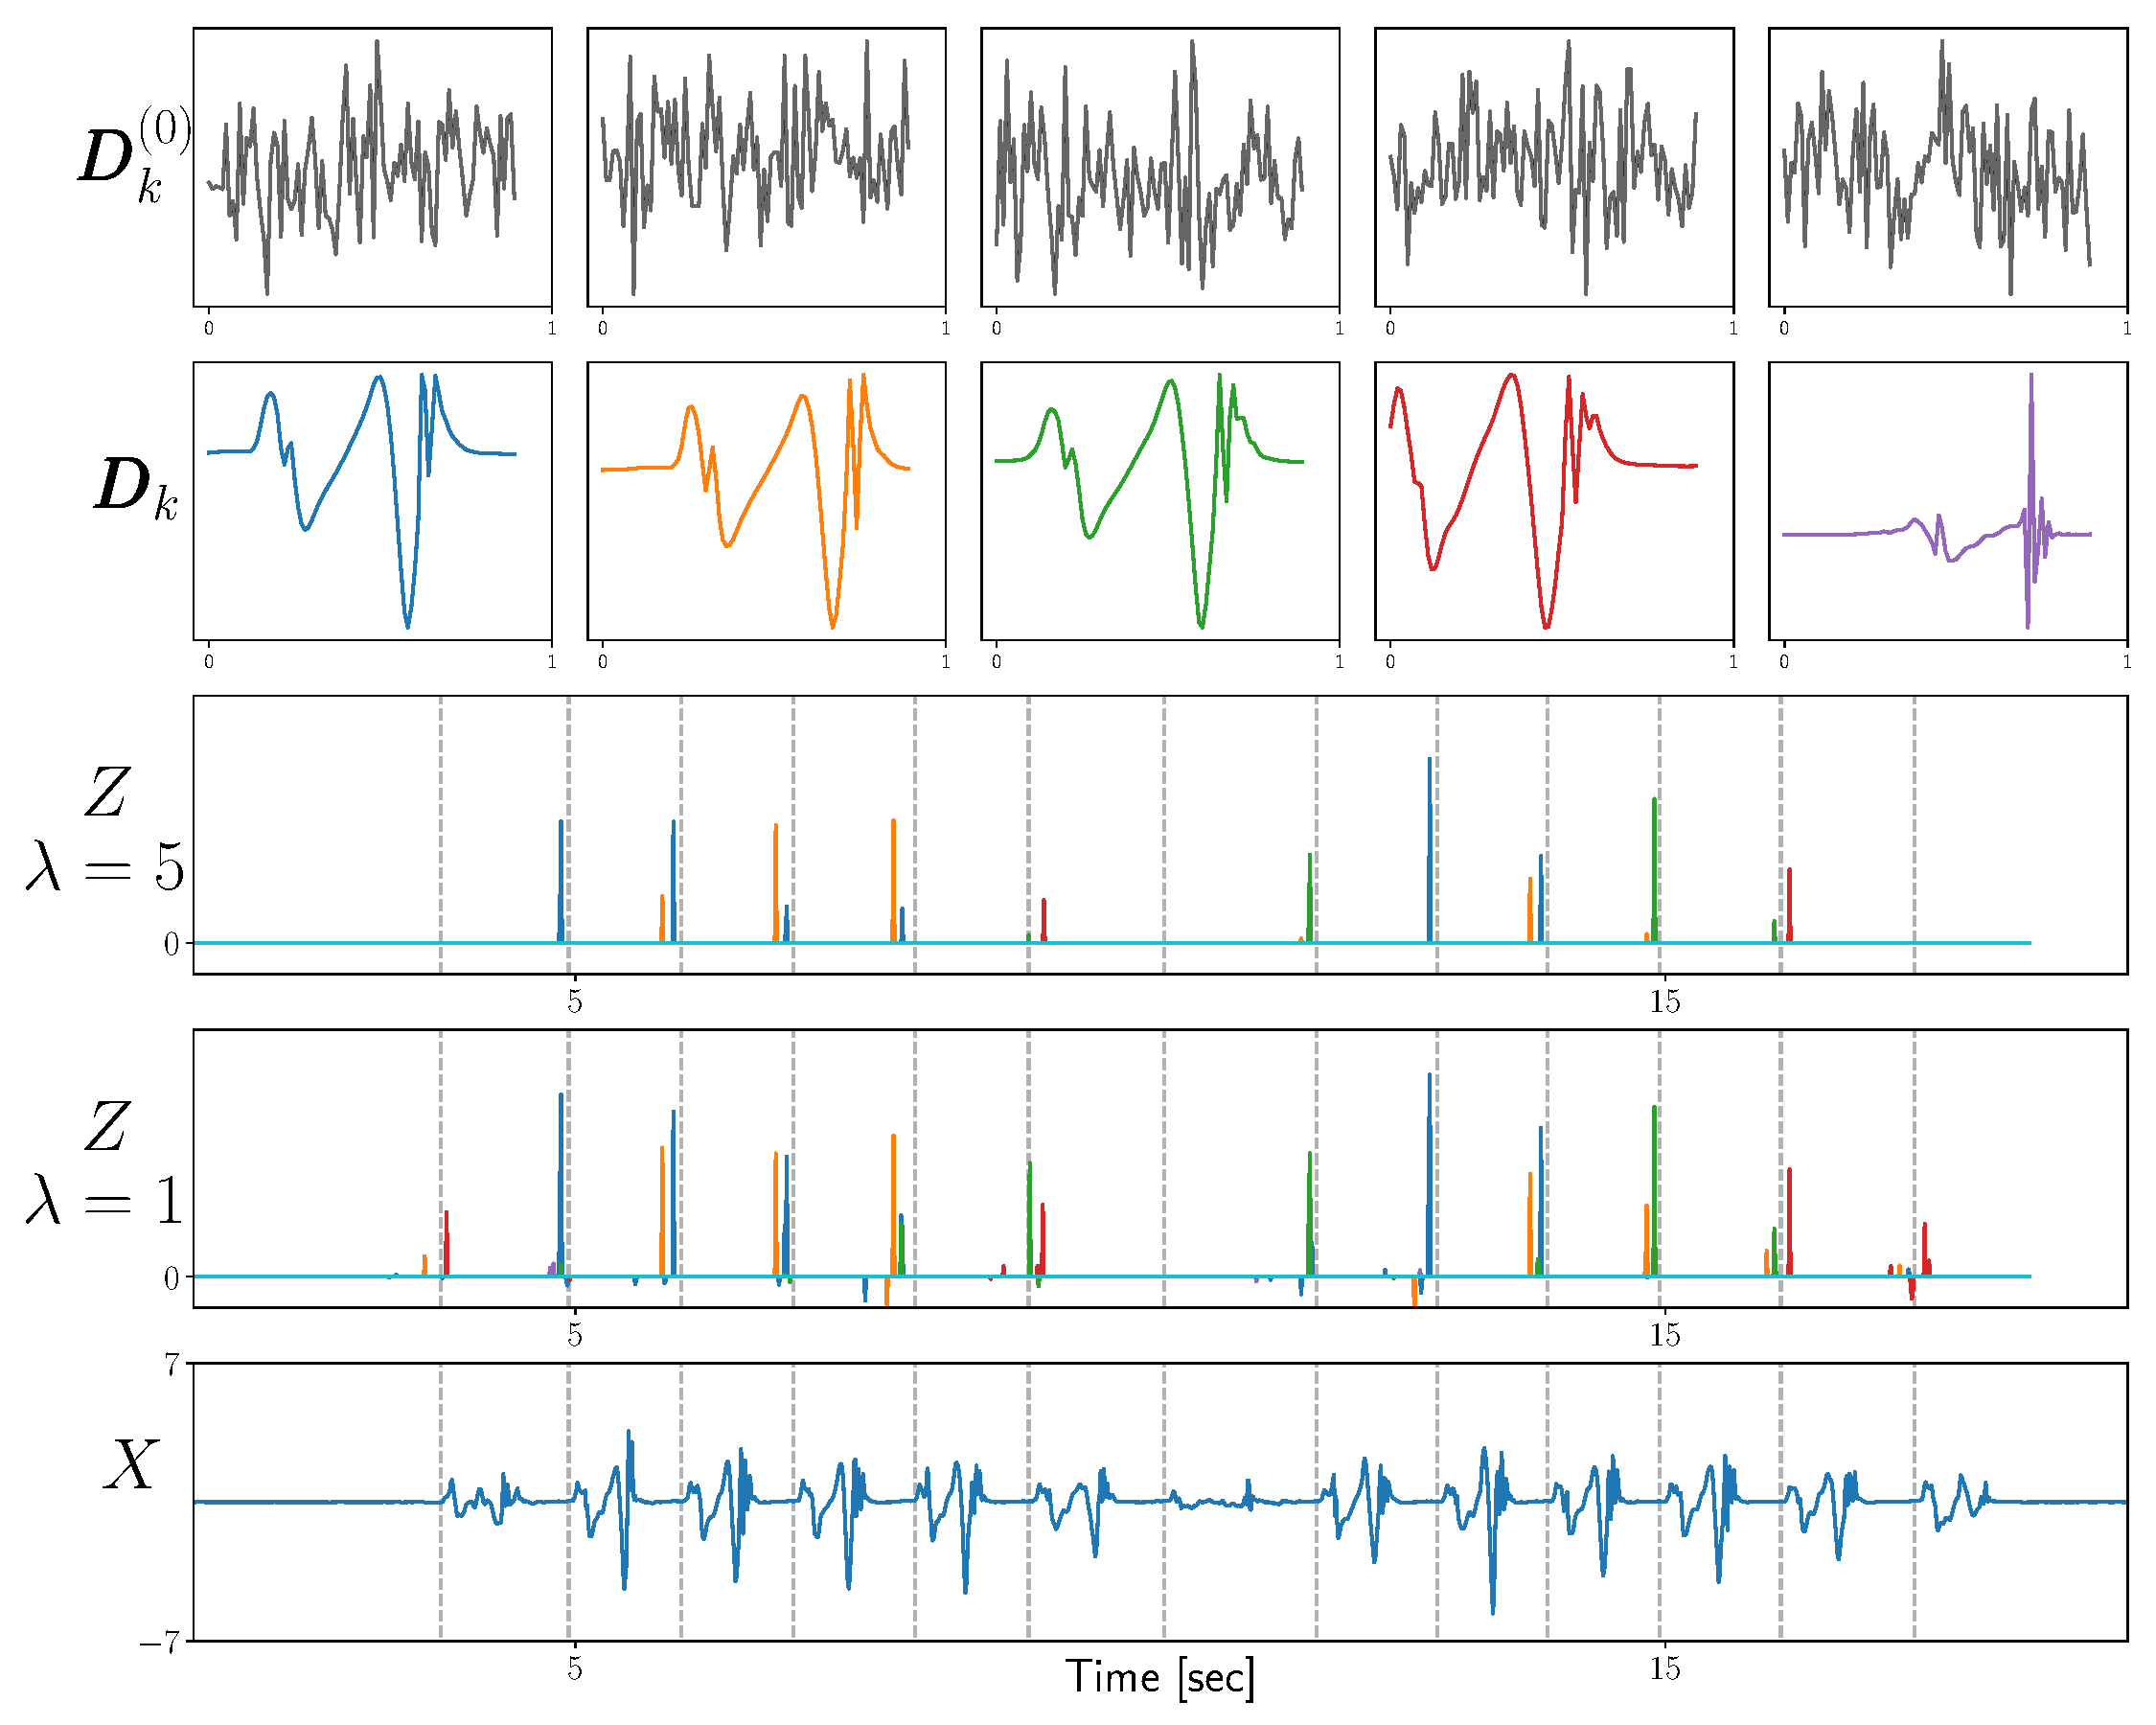
\includegraphics[width=.8\textwidth]{csc_random_defense}

\end{frame}


\begin{frame}
	\centering
	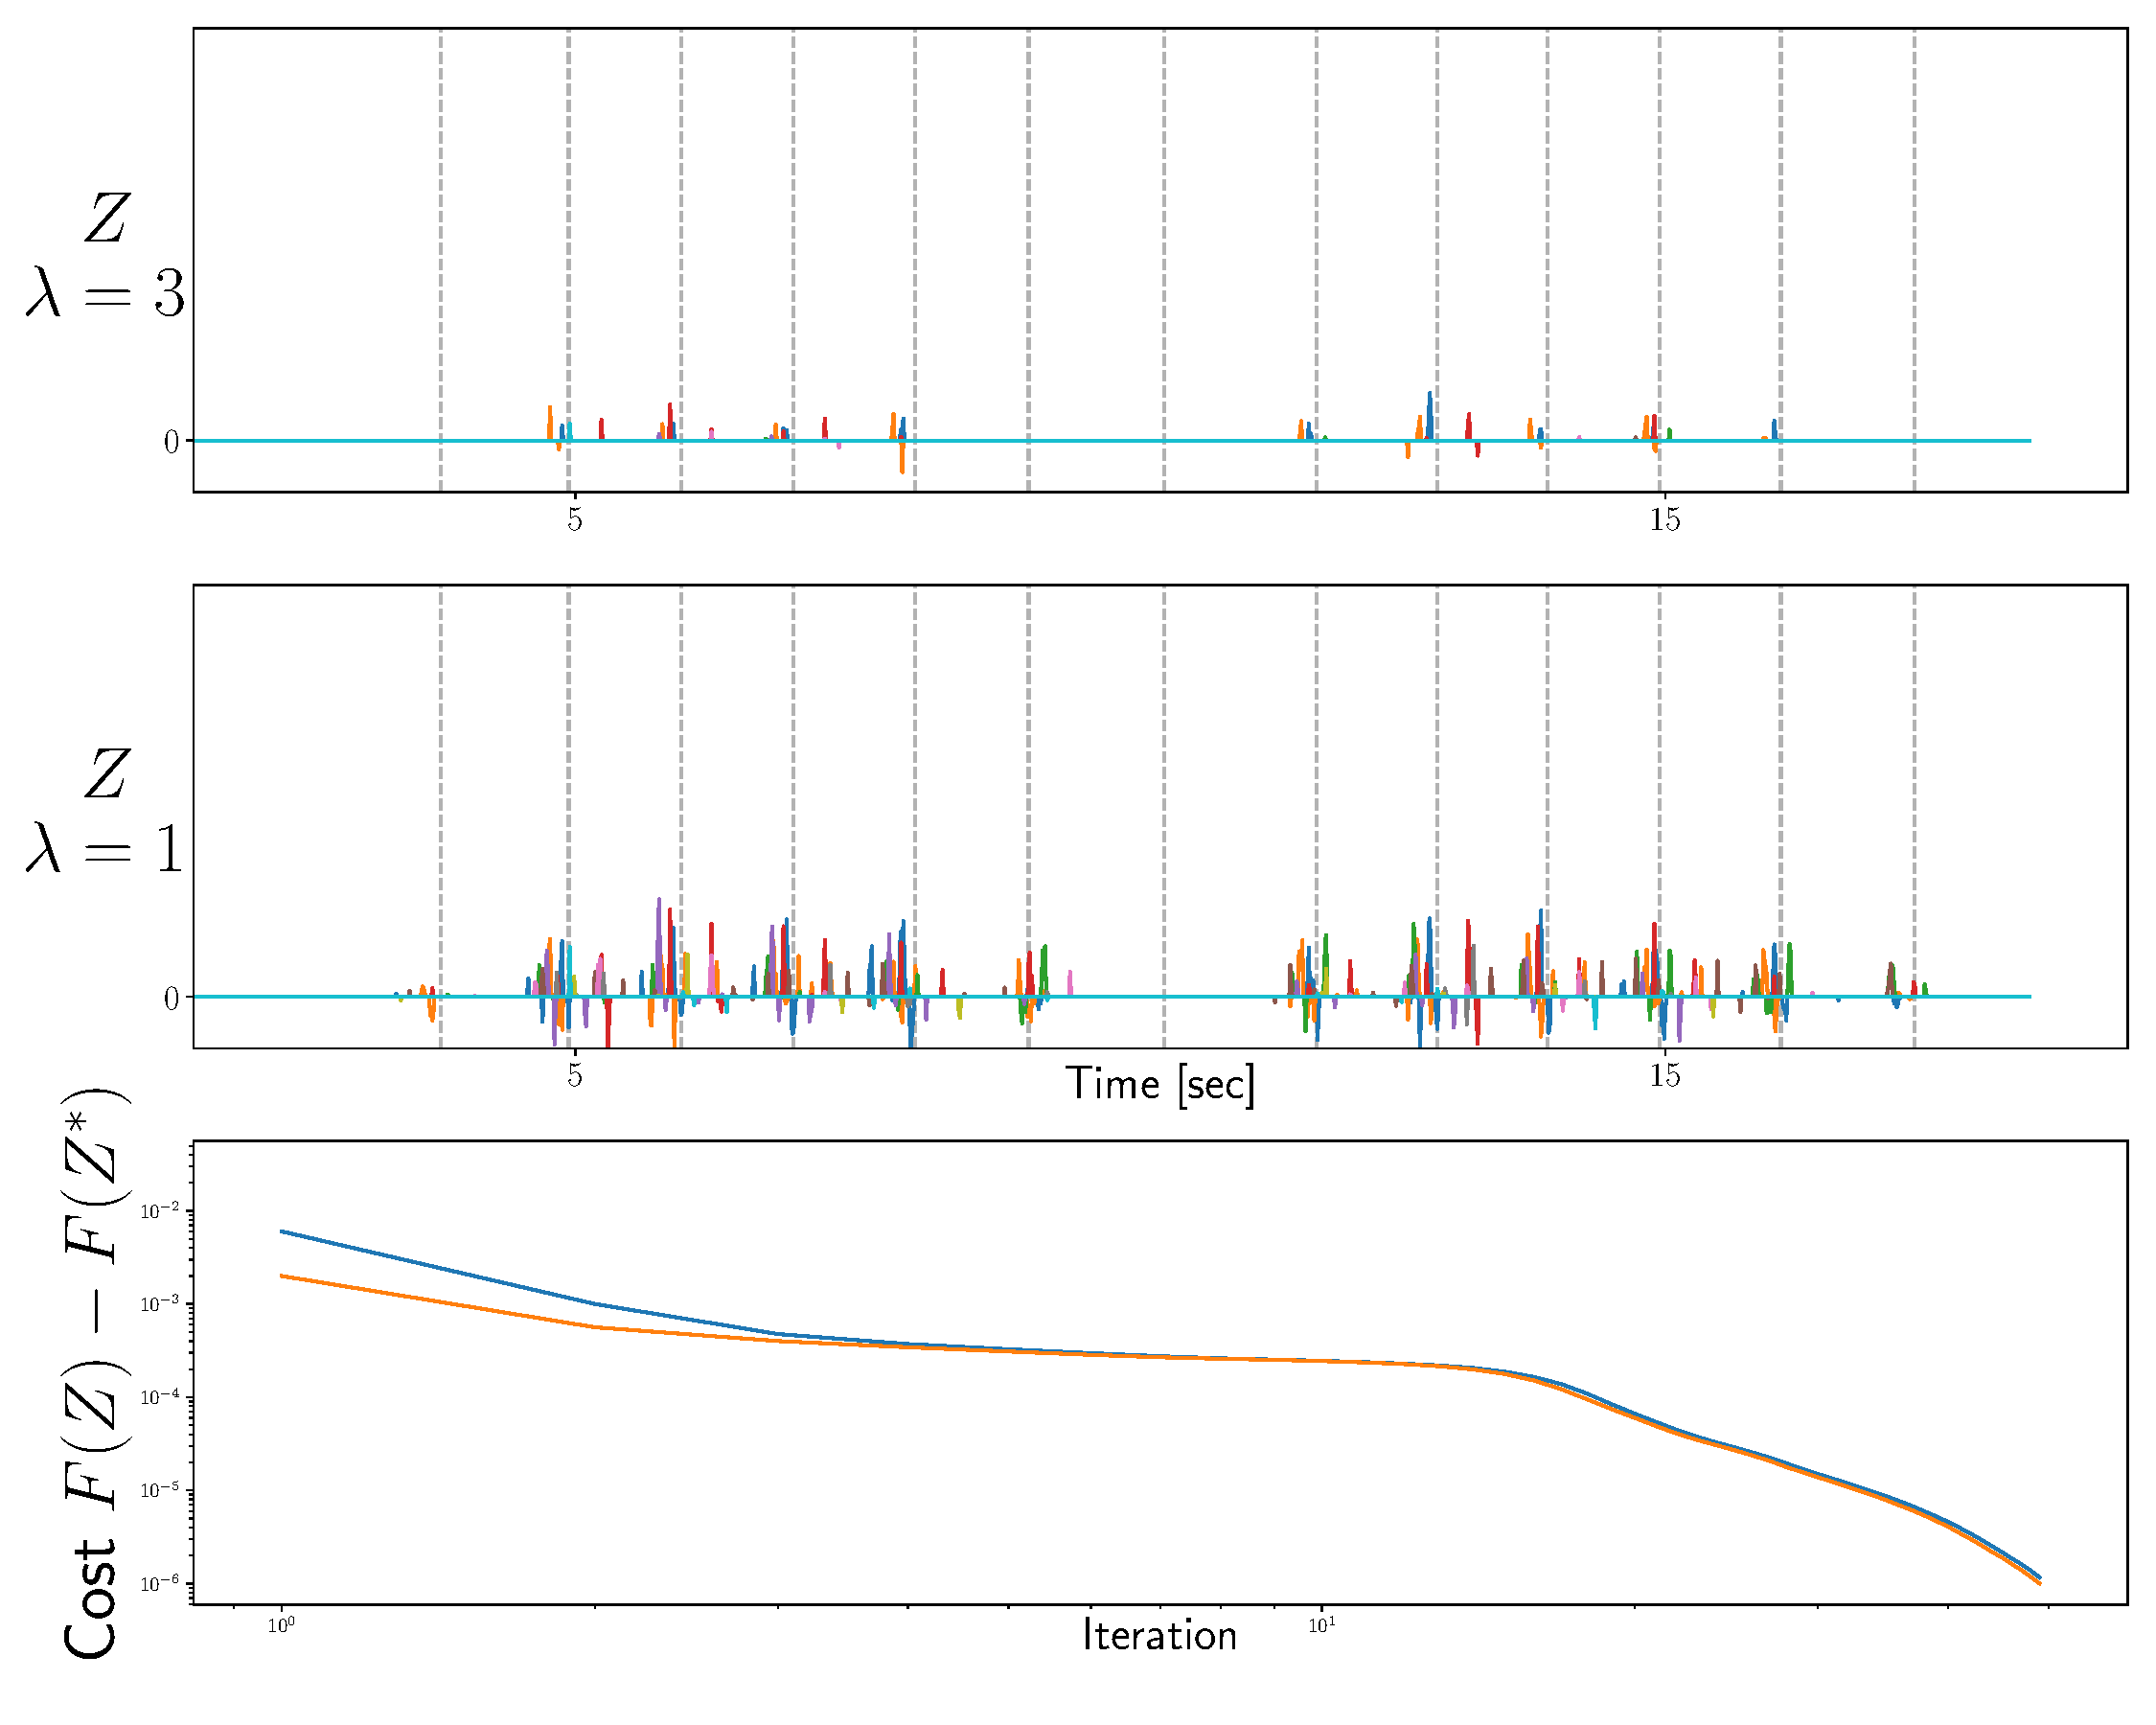
\includegraphics[width=.8\textwidth]{csc_random_annex}	
\end{frame}

%====================================================================
\subsection{DICOD}
%====================================================================

\begin{frame}{Finishing the process in a distributed environment}


	Non trivial point: {\bf How to decide that the algorithm has converged?}\\[2em]
	
	\begin{itemize}\itemsep2em\itemindent1em
		\item Neighbors paused is not enough!
		\item Define a master 0 and send probes.\\
			\hskip3em Wait for $M$ probes return.
		\item Uses the notion of message queue and network flow.\\
			\hskip3em Maybe we can have better way?
	\end{itemize}
	
	
\end{frame}


\begin{frame}
\frametitle{Numerical Experiments}


\definecolor{fista}{RGB}{192,192,0}
\definecolor{rcd}{RGB}{0,128,0}
\definecolor{cd}{RGB}{255, 0, 0}
\definecolor{dicod}{RGB}{0,0,255}

Test on long signals generated with Bernoulli-Gaussian
coding signal $Z$ and a Gaussian dictionary $\pmb D$.
Fixed $K = 25$, $W = 200$ and $T = 600*W$,\\[1em]

\textbf{Algorithms implemented for benchmark}
\begin{itemize}
    \item {\color{cd} Coordinate Descent} (CD) \\\mycite{Kavukcuoglu2013}
    \item {\color{rcd} Randomized Coordinate Descent} (RCD) \\\mycite{Nesterov2010}
    \item Fast Convolutional Sparse Coding (FCSC)\\\mycite{Bristow2013}
    \item {\color{fista}Fast Ierative Soft-Thresholding Algorithm (FISTA)} \\\mycite{Chalasani2013, Wohlberg2016}
    \item {\color{dicod} DICOD with $60$ cores}
\end{itemize}
\end{frame}


\begin{frame}{Numerical convergence}

\centering
\alt<2>{
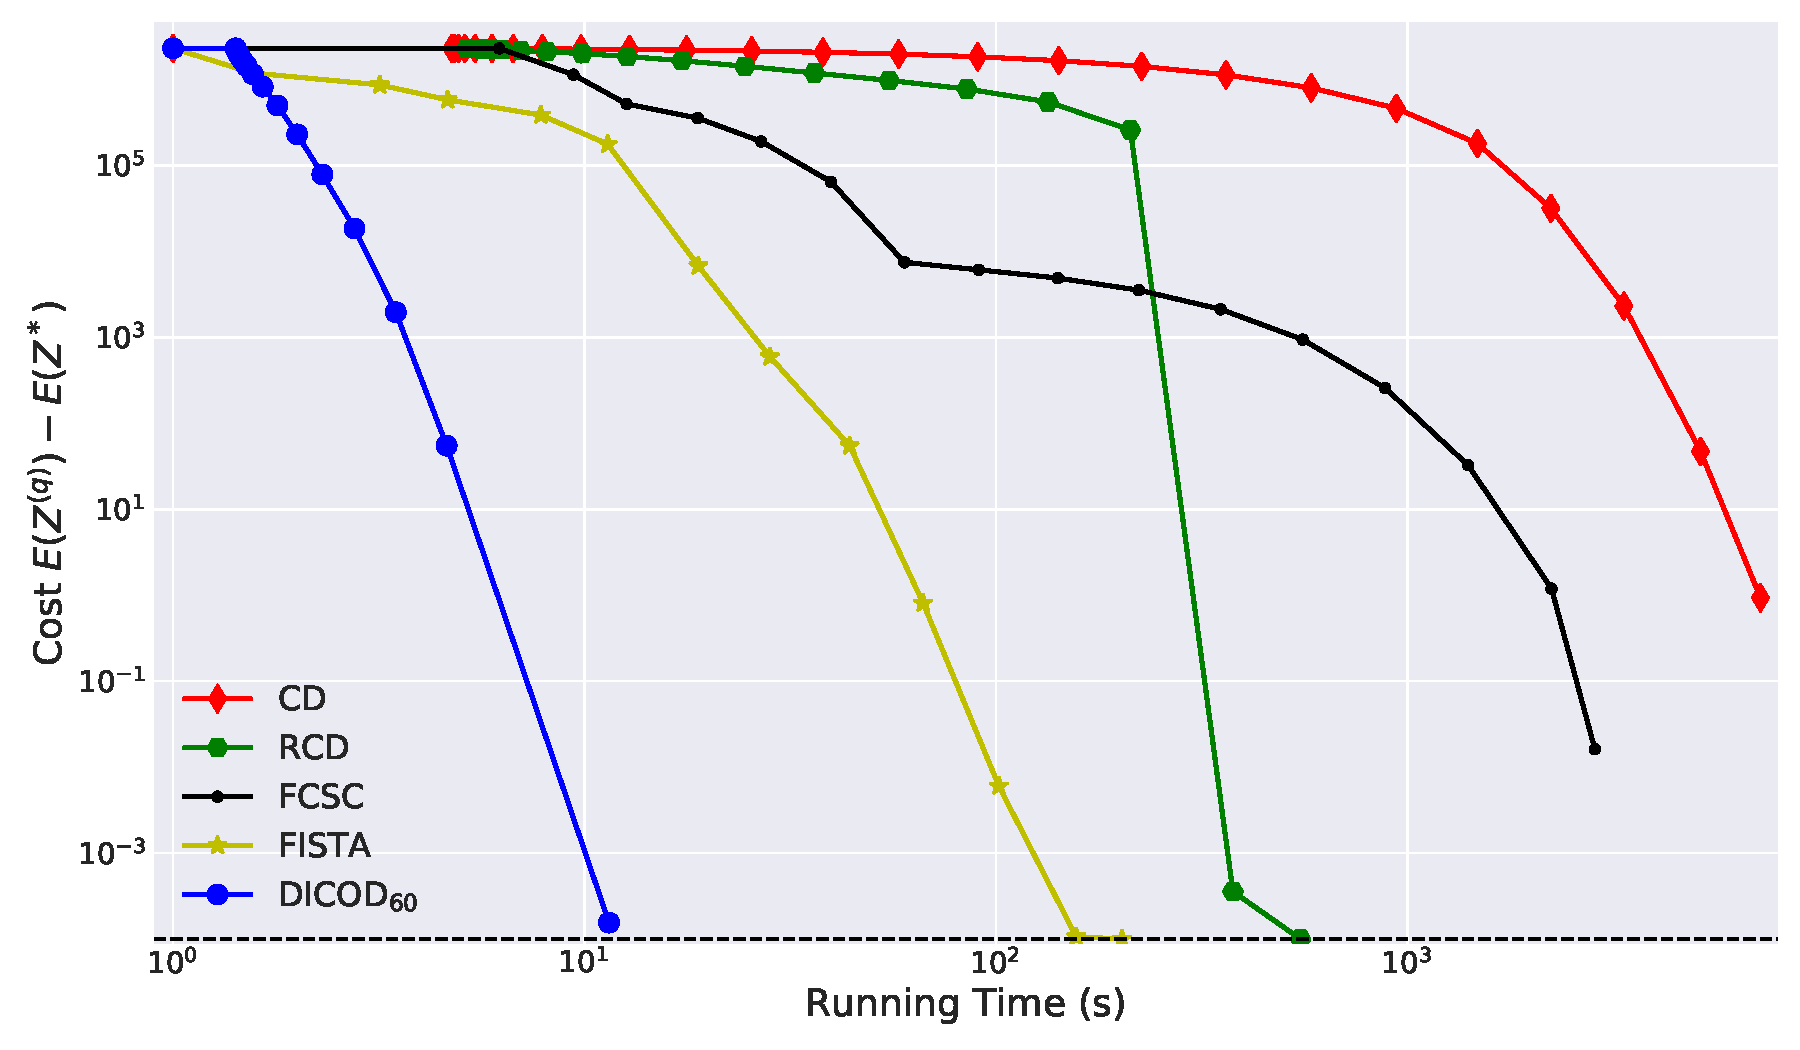
\includegraphics[width=.8\textwidth]{cost_min_seaborn_time}\\
\large Cost as a function of the runtime\\
}{
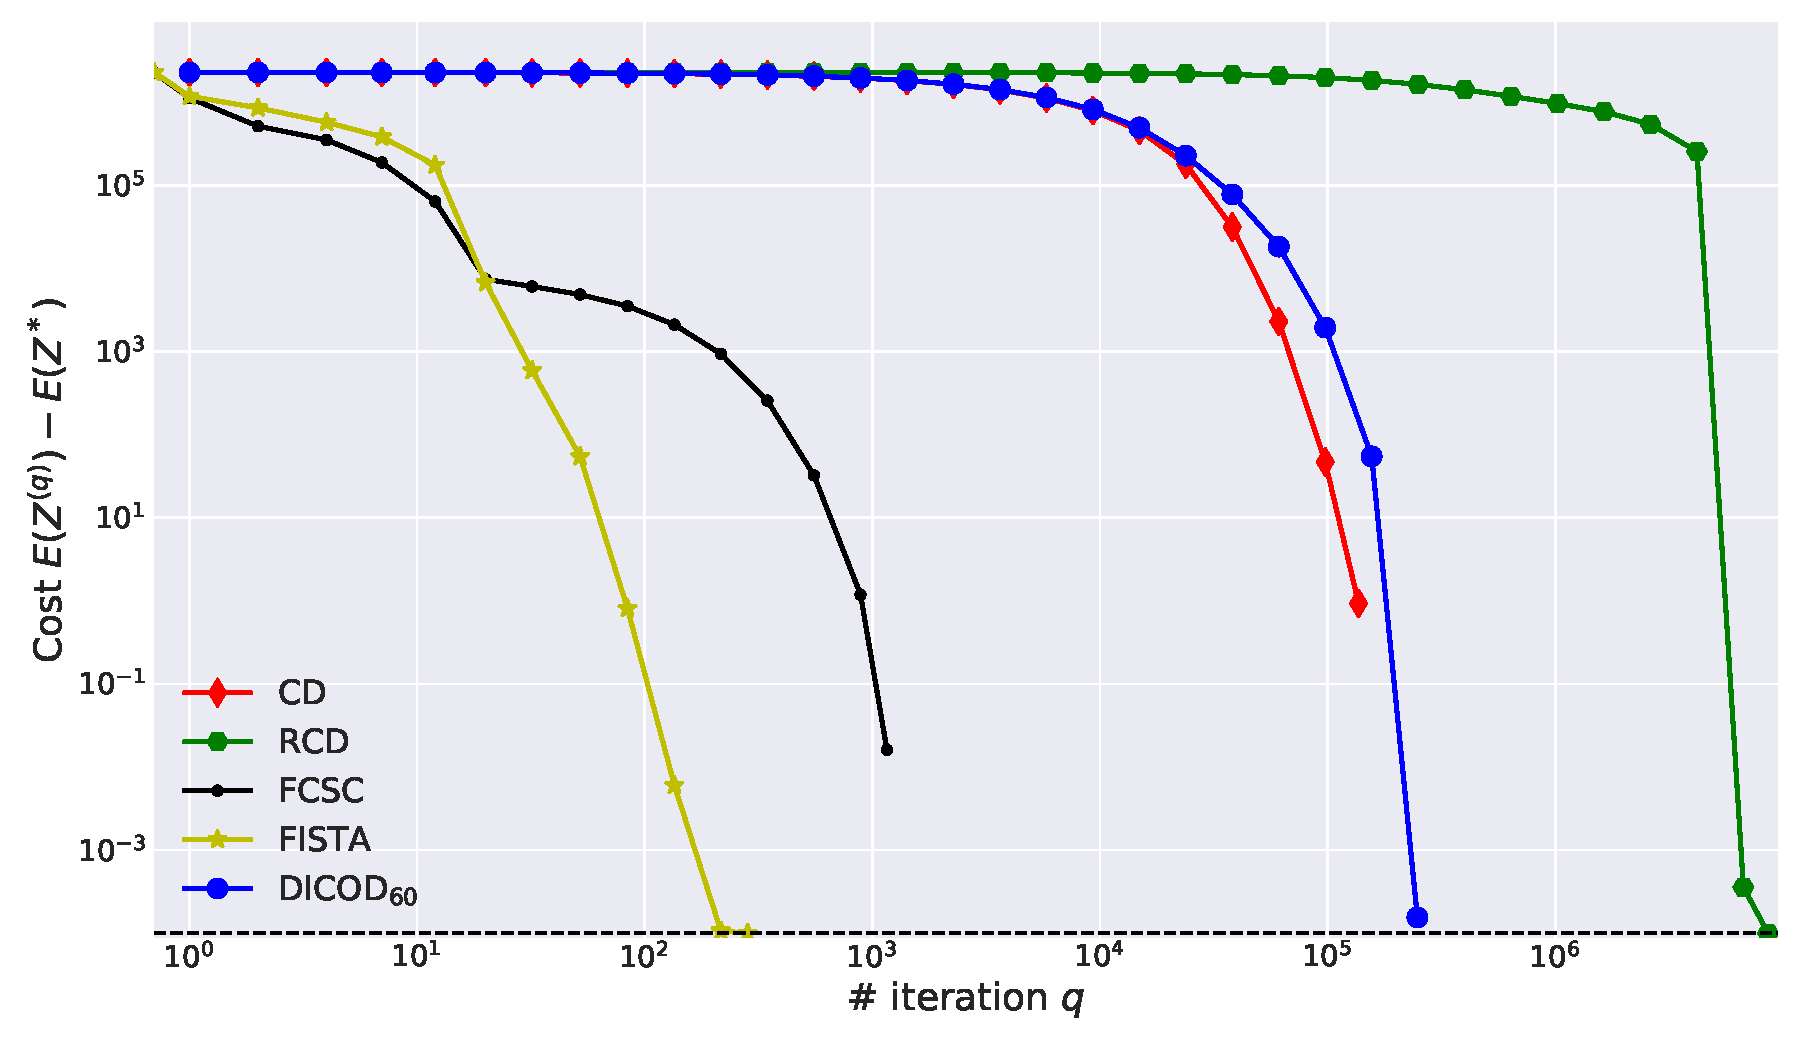
\includegraphics[width=.8\textwidth]{cost_min_seaborn_iter}\\
\large Cost as a function of the iterations\\
}
\end{frame}



\begin{frame}{DICOD: numerical convergence}
	\alt<2>{
		\centering
		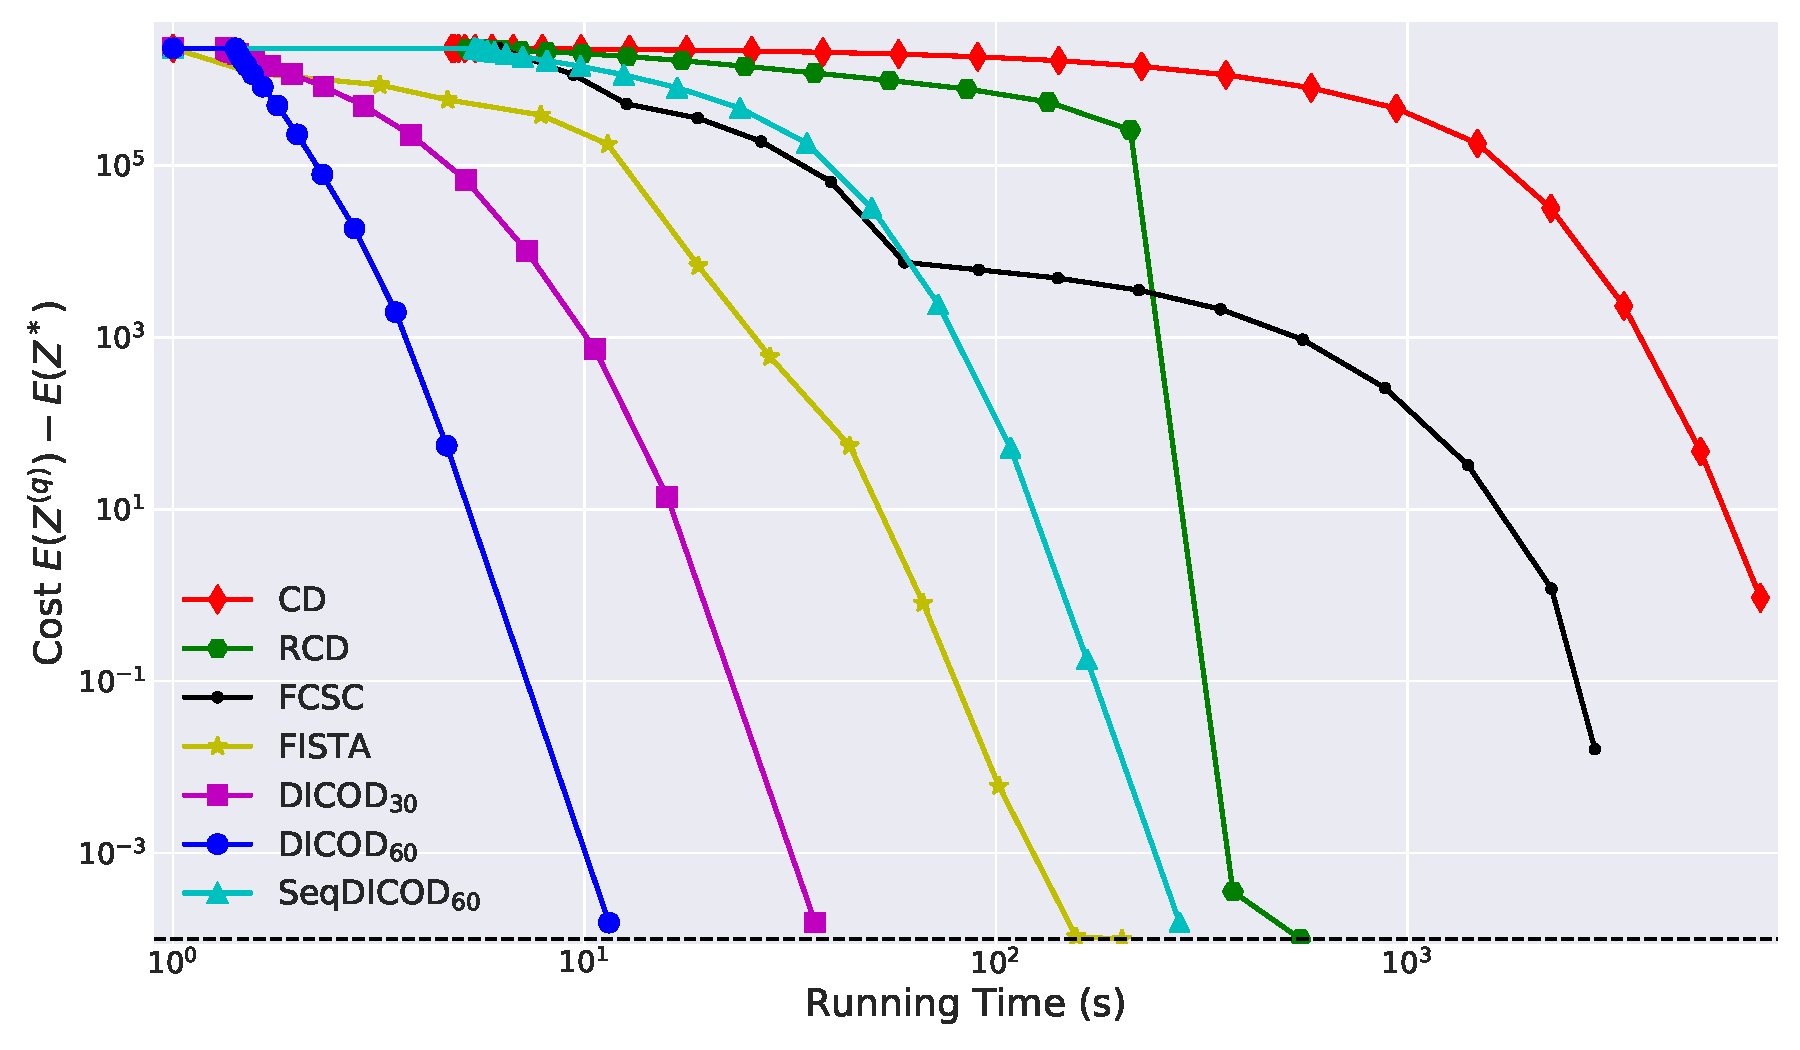
\includegraphics[width=\textwidth]{cost_seaborn_time}\\
		\large Cost as a function of the time
	}{
        \centering
        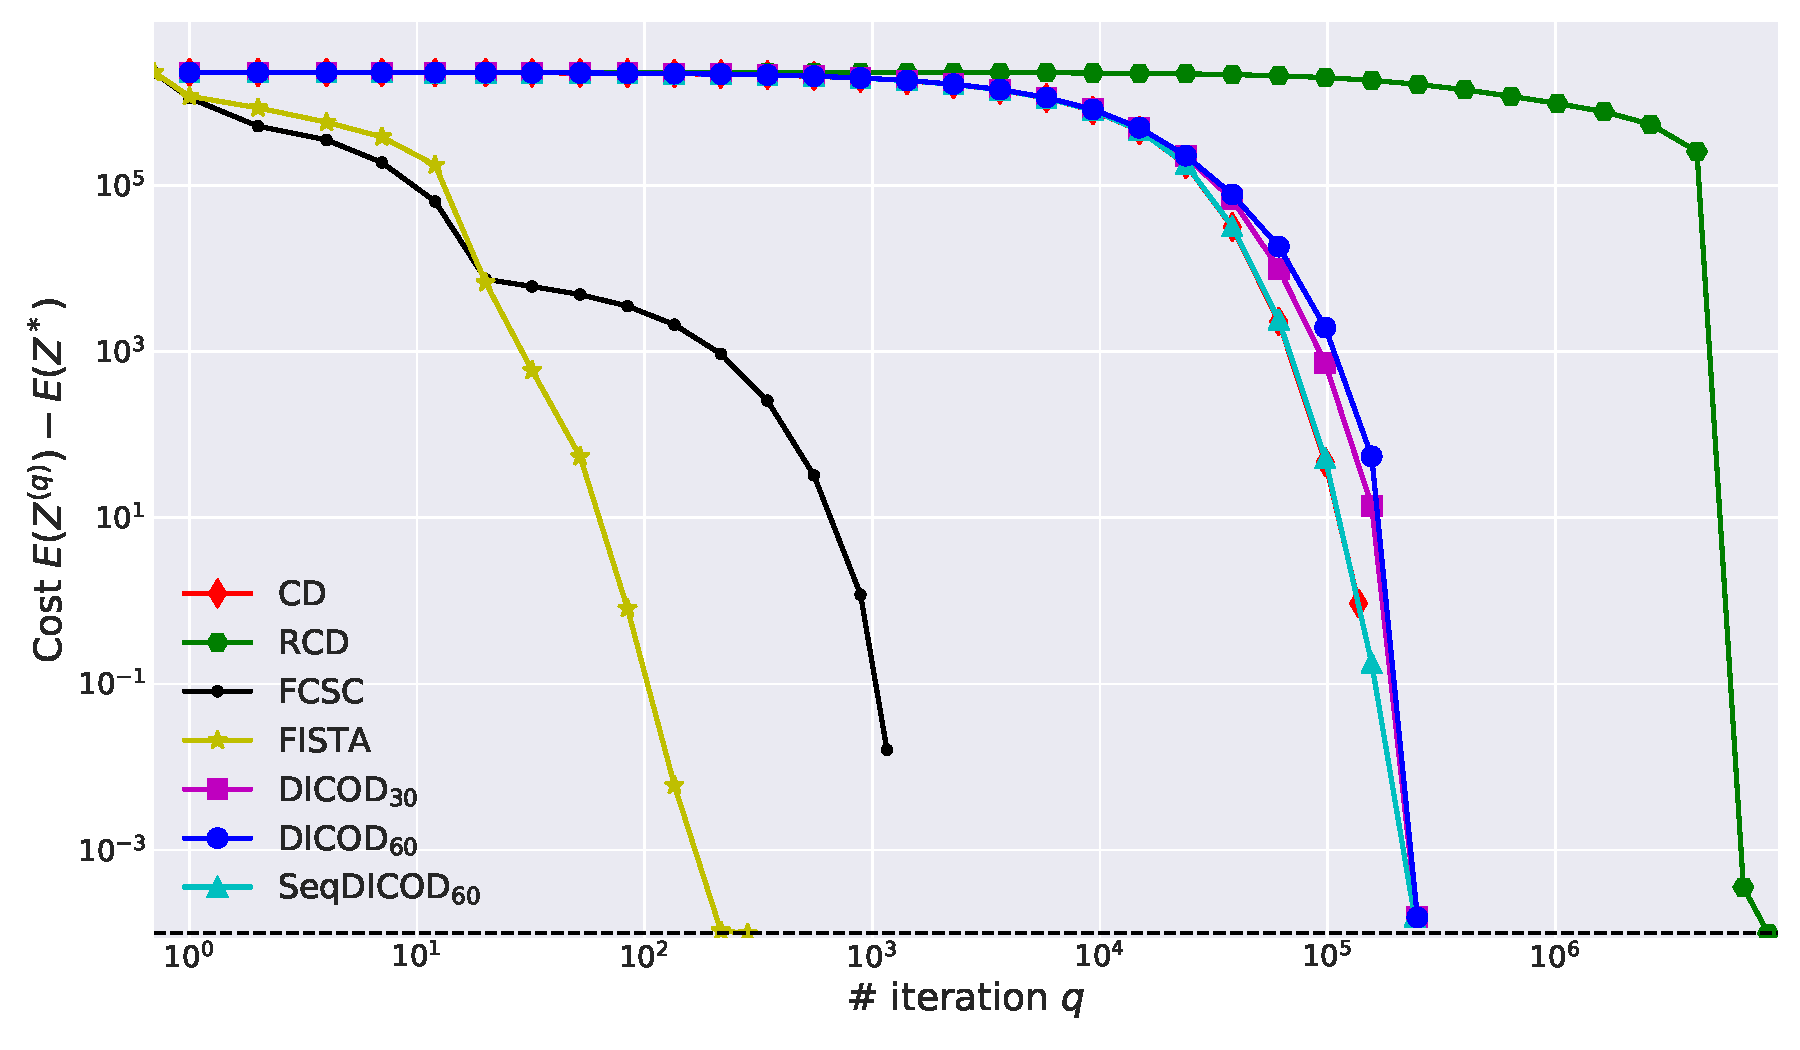
\includegraphics[width=\textwidth]{cost_seaborn_iter}\\
        \large Cost as a function of the iterations
    }
\end{frame}


\begin{frame}{Complexity Analysis}
Two sources of acceleration:\\[1em]
\begin{itemize}\itemsep1em
    \item Perform $M$ updates in parallel,
    \item Each update is computed on a segment of size $\frac{L}{M}$\\
    Iteration complexity of $\bO{K\frac{L}{M}}$ instead of $\bO{KL}$ 
\end{itemize}
\vskip1em
Limitations:
\begin{itemize}
    \item Interfering updates, with probability $\alpha^2 = \left(\frac{WM}{T}\right)^2$
    \[
    \mathbb E[Q_{dicod}] \smeq\underset{\alpha \to 0}{\gtrsim}
    M(1-2\alpha^2M^2 + \mathcal O(\alpha^4M^4))~.
    \]
    \item Cost of the update of $\beta$ in $\bO{KW}$  
\end{itemize}

\end{frame}

\end{document}
